\documentclass[12pt]{article}

\usepackage{amsmath, mathtools}
\usepackage{amsfonts}
\usepackage{amssymb}
\usepackage{graphicx}
\usepackage{colortbl}
\usepackage{xr}
\usepackage{hyperref}
\usepackage{longtable}
\usepackage{xfrac}
\usepackage{tabularx}
\usepackage{float}
\usepackage{siunitx}
\usepackage{booktabs}
\usepackage{caption}
\usepackage{pdflscape}
\usepackage{afterpage}

\usepackage[round]{natbib}

\usepackage{titlesec}

%\usepackage{refcheck}

\hypersetup{
    bookmarks=true,         % show bookmarks bar?
      colorlinks=true,       % false: boxed links; true: colored links
    linkcolor=red,          % colour of internal links (change box colour with linkbordercolor)
    citecolor=green,        % colour of links to bibliography
    filecolor=magenta,      % colour of file links
    urlcolor=cyan           % colour of external links
}

%% Comments
\usepackage{color}
\newif\ifcomments\commentstrue %displays comments
%\newif\ifcomments\commentsfalse %so that comments do not display
\ifcomments
\newcommand{\authornote}[3]{\textcolor{#1}{[#3 ---#2]}}
\newcommand{\todo}[1]{\textcolor{red}{[TODO: #1]}}
\else
\newcommand{\authornote}[3]{}
\newcommand{\todo}[1]{}
\fi
\newcommand{\wss}[1]{\authornote{blue}{SS}{#1}} 
\newcommand{\plt}[1]{\authornote{magenta}{TPLT}{#1}} %For explanation of the template
\newcommand{\an}[1]{\authornote{cyan}{Author}{#1}}
%% Common Parts
\newcommand{\progname}{4TB6 - Mechatronics Capstone} % PUT YOUR PROGRAM NAME HERE
\newcommand{\authname}{Team \#5, Locked \& Loaded
\\ Abi Nevo, nevoa
\\ Elsa Bassi, bassie
\\ Steffi Ralph, ralphs1
\\ Abdul Iqbal, iqbala18
\\ Stephen De Jong, dejons1
\\ Anthony Shenouda, shenoa2} % AUTHOR NAMES                  

\usepackage{hyperref}
    \hypersetup{colorlinks=true, linkcolor=blue, citecolor=blue, filecolor=blue,
                urlcolor=blue, unicode=false}
    \urlstyle{same}


% For an easy change of table widths
\newcommand{\colZwidth}{1.0\textwidth}
\newcommand{\colAwidth}{0.13\textwidth}
\newcommand{\colBwidth}{0.82\textwidth}
\newcommand{\colCwidth}{0.1\textwidth}
\newcommand{\colDwidth}{0.05\textwidth}
\newcommand{\colEwidth}{0.8\textwidth}
\newcommand{\colFwidth}{0.17\textwidth}
\newcommand{\colGwidth}{0.5\textwidth}
\newcommand{\colHwidth}{0.28\textwidth}

% Used so that cross-references have a meaningful prefix
\newcounter{defnum} %Definition Number
\newcommand{\dthedefnum}{GD\thedefnum}
\newcommand{\dref}[1]{GD\ref{#1}}
\newcounter{datadefnum} %Datadefinition Number
\newcommand{\ddthedatadefnum}{DD\thedatadefnum}
\newcommand{\ddref}[1]{DD\ref{#1}}
\newcounter{theorynum} %Theory Number
\newcommand{\tthetheorynum}{T\thetheorynum}
\newcommand{\tref}[1]{T\ref{#1}}
\newcounter{tablenum} %Table Number
\newcommand{\tbthetablenum}{T\thetablenum}
\newcommand{\tbref}[1]{TB\ref{#1}}
\newcounter{assumpnum} %Assumption Number
\newcommand{\atheassumpnum}{P\theassumpnum}
\newcommand{\aref}[1]{A\ref{#1}}
\newcounter{goalnum} %Goal Number
\newcommand{\gthegoalnum}{P\thegoalnum}
\newcommand{\gsref}[1]{GS\ref{#1}}
\newcounter{scnum} %System Constraint Number
\newcommand{\scthescnum}{SC\thscnum}
\newcommand{\scref}[1]{SC\ref{#1}}
\newcounter{instnum} %Instance Number
\newcommand{\itheinstnum}{IM\theinstnum}
\newcommand{\iref}[1]{IM\ref{#1}}
\newcounter{reqnum} %Requirement Number
\newcommand{\rthereqnum}{P\thereqnum}
\newcommand{\rref}[1]{R\ref{#1}}
\newcounter{nfrnum} %NFR Number
\newcommand{\rthenfrnum}{NFR\thenfrnum}
\newcommand{\nfrref}[1]{NFR\ref{#1}}
\newcounter{lcnum} %Likely change number
\newcommand{\lthelcnum}{LC\thelcnum}
\newcommand{\lcref}[1]{LC\ref{#1}}
\newcounter{ulcnum} %Unlikely change number
\newcommand{\ltheulcnum}{ULC\theulcnum}
\newcommand{\ulcref}[1]{ULC\ref{#1}}
\newcounter{constnum} %Unlikely change number
\newcommand{\ltheconstnum}{CONST\theconstnum}
\newcommand{\constref}[1]{CONST\ref{#1}}

\usepackage{fullpage}

\newcommand{\deftheory}[9][Not Applicable]
{
\newpage
\noindent \rule{\textwidth}{0.5mm}

\paragraph{RefName: } \textbf{#2} \phantomsection 
\label{#2}

\paragraph{Label:} #3

\noindent \rule{\textwidth}{0.5mm}

\paragraph{Equation:}

#4

\paragraph{Description:}

#5

\paragraph{Notes:}

#6

\paragraph{Source:}

#7

\paragraph{Ref.\ By:}

#8

\paragraph{Preconditions for \hyperref[#2]{#2}:}
\label{#2_precond}

#9

\paragraph{Derivation for \hyperref[#2]{#2}:}
\label{#2_deriv}

#1

\noindent \rule{\textwidth}{0.5mm}

}

%\documentclass{article}


\setcounter{secnumdepth}{4}

\titleformat{\paragraph}
{\normalfont\normalsize\bfseries}{\theparagraph}{1em}{}
\titlespacing*{\paragraph}
{0pt}{3.25ex plus 1ex minus .2ex}{1.5ex plus .2ex}


\begin{document}

\title{Software Requirements Specification for SmartLock\\\progname} 
\author{\authname}
\date{\today}
	
\maketitle
\thispagestyle{empty}
\begin{figure}[h!]
  \centering
  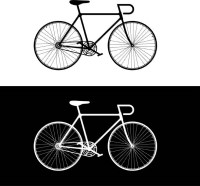
\includegraphics[width=0.4\linewidth]{../BikeLogo.jpg}
\end{figure}

\newpage
\pagenumbering{roman}
\begin{table}[hp]
\caption{Revision History} \label{TblRevisionHistory}
\begin{tabularx}{\textwidth}{llX}
\toprule
\textbf{Date} & \textbf{Developer(s)} & \textbf{Change}\\
\midrule
02-10-22 & Elsa & Drafted first draft\\
03-10-22 & Stephen & Drafted 1 \& 5, and formatting updates\\
03-10-22 & Abi & Drafted Likely and Unlikely Changes\\
04-10-22 & Steffi & Drafted Appendix\\
04-10-22 & Abi & Drafted Dev Plan and added Reflection\\
04-10-22 & Steffi & Added Reflections and Section 3 Removed unnecessary subsections from Section 4 added traceability\\
14-10-22 & Abi & Fixed System Constraint numbering\\
19-11-22 & Steffi & Updates for Consistency\\
26-01-23 & Elsa & Updates as per Peer Reviews and Further Consistency\\
\bottomrule
\end{tabularx}
\end{table}

\newpage


\tableofcontents

\newpage
\pagenumbering{arabic}
\section{Reference Material}

This section records information for easy reference.

\subsection{Table of Units}

Throughout this document, SI (Syst\`{e}me International d'Unit\'{e}s) is employed
as the unit system.  In addition to the basic units, several derived units are
used as described below.  For each unit, the symbol is given followed by a
description of the unit and the SI name.
~\newline

\renewcommand{\arraystretch}{1.2}
%\begin{table}[ht]
%\begincenter
  \noindent \begin{tabular}{l l l} 
    \toprule		
    \textbf{symbol} & \textbf{unit} & \textbf{SI}\\
    \midrule 
    \si{\metre} & length & metre\\
    \si{\kilogram} & mass	& kilogram\\
    \si{\second} & time & second\\
    \si{\joule} & energy & joule\\
    P or \si{\watt} & power & watt (W = \si{\joule\per\second})\\
    \si{\ampere} or I& current & ampere\\
    \si{\ohm} or R& resistance & ohm\\
    \si{\volt} & voltage & volt\\
    \si{\newton} & force & newton\\
    \si{\newton}M & torque & newton meter\\
    \bottomrule
  \end{tabular}
  %	\caption{Provide a caption}
%\end{table}

\subsection{Table of Symbols}

The table that follows summarizes the symbols used in this document along with
their units.  The choice of symbols was made to be consistent with the heat
transfer literature and with existing documentation for solar water heating
systems.  The symbols are listed in alphabetical order.

\renewcommand{\arraystretch}{1.2}
%\noindent \begin{tabularx}{1.0\textwidth}{l l X}
\noindent \begin{longtable*}{l l p{12cm}} \toprule
\textbf{symbol} & \textbf{unit} & \textbf{description}\\
\midrule 
$B_L$ & hour & battery life in hours\\
$B_C$ & mAH & battery capacity in amp hours\\
$L_C$ & A/actuation & current drawn per motor actuation\\
$A_\text{num}$ & actuation/charge & number of actuations per charge\\ 
\bottomrule
\end{longtable*}


\subsection{Abbreviations and Acronyms}

\renewcommand{\arraystretch}{1.2}
\begin{tabular}{l l} 
  \toprule		
  \textbf{symbol} & \textbf{description}\\
  \midrule 
  SRS & Software Requirements Specification\\
  FR & Functional Requirements\\
  NFR & Nonfunctional Requirements\\
  LC & Likely Changes\\
  ULC & Unlikely Changes\\
  SC & System Contraints\\
  A & Assumptions\\
  MV & Monitored Variables\\
  \bottomrule
\end{tabular}\\


%\subsection{Mathematical Notation}




\section{Introduction}

The purpose of the SmartLock project is to design and build a product that will provide bicycle users with a safer, easier, and more accessible way to secure their bike(s) through their smartphone. Additionally, it will provide users with a GPS feature to locate the lock in case of bike theft or misplacement.  It will consist of a physical lock that mounts to a bike and a smartphone application that will function as the user interface through which the lock can be engaged and disengaged wirelessly, as well as located. The project will provide an engineering solution using wireless communication, mechanical design, and smartphone application development. More broadly, it seeks to encourage members of society to pursue biking, in both a transportation and recreational capacity, improving the health of society’s citizens and its environment.  

\subsection{Purpose of Document}

The Requirements Documentation seeks to provide a complete overview of the requirements of the SmartLock system so as to define the project. The assumptions, inputs and outputs will also be defined in order to outline the problem. Several models will be developed and lastly, likely and unlikely changes will be described. This will communicate a unified and documented plan for the project that can be used after the design stage to verify its functionality and provide an important benchmark. 

\subsection{Scope of Requirements} 

The SmartLock project will build off existing designs to tie together principles of wireless communication, GPS, a mechanical locking mechanism, electrical actuation, and smartphone application development. The system will provide all functions necessary for effective and secure locking and location.  

The SmartLock project will be designed to perform the following functions for the user.  

\begin{enumerate}
\item Wireless communication from the smartphone to the lock and vice versa. 
\item Display of lock and battery status information on the App. 
\item Display of location on the App. 
\item Store and use a replaceable battery. 
\item House a mechanical lock frame. 
\item Perform electrical engagement/disengagement of a locking mechanism. 
\item Be waterproof. 
\end{enumerate}

Not included in the project scope will be a fully autonomous lock frame, (only the disengagement function will be automated), and a rechargeable battery. We will also be ignoring extreme weather and temperature conditions and their impact on the material properties.

\subsection{Characteristics of Intended Reader} \label{sec_IntendedReader}

The reader will have basic knowledge of how bikes are secured in public settings, namely using mechanical locks and keys or combination locks. They will understand why bike locking is necessary and what it means for a bike to be vulnerable to theft, i.e. that all main parts of the bike must be secured including the frame and wheels. They will also have basic knowledge of wireless communications that can be accessed through smartphone applications. Lastly, the reader will have a high-school-level understanding of kinematic and electronics-related physics and math such that they can grasp the mechanical and electrical functionality of the system.  

\subsection{Organization of Document}

The document will follow the base template provided by the Capstone 4TB6 course GitLab. It will be organized with increasing order of specificity, beginning with the General System Description which will include an overview of the SmartLock project. The Specific System Description will make up the bulk of the document, describing the project in greater detail with its assumptions, inputs and outputs, goals and models. Finally, since the context of the project is previously stated, the Functional and Non-Functional Requirements will be outlined, as well as any foreseen Likely and Unlikely Changes to the project. Lastly, the Traceability Matrix is included to define the relationships between various relevant formulas, sections and information in the document and how they are used to build the project.  

~\newpage

\section{General System Description}

This section provides general information about the system. It identifies the interfaces between the system and its environment describes the user characteristics and lists the system constraints.  

\subsection{System Context}

 \begin{figure}[h!]
 \begin{center}
 %\rotatebox{-90}
 {
  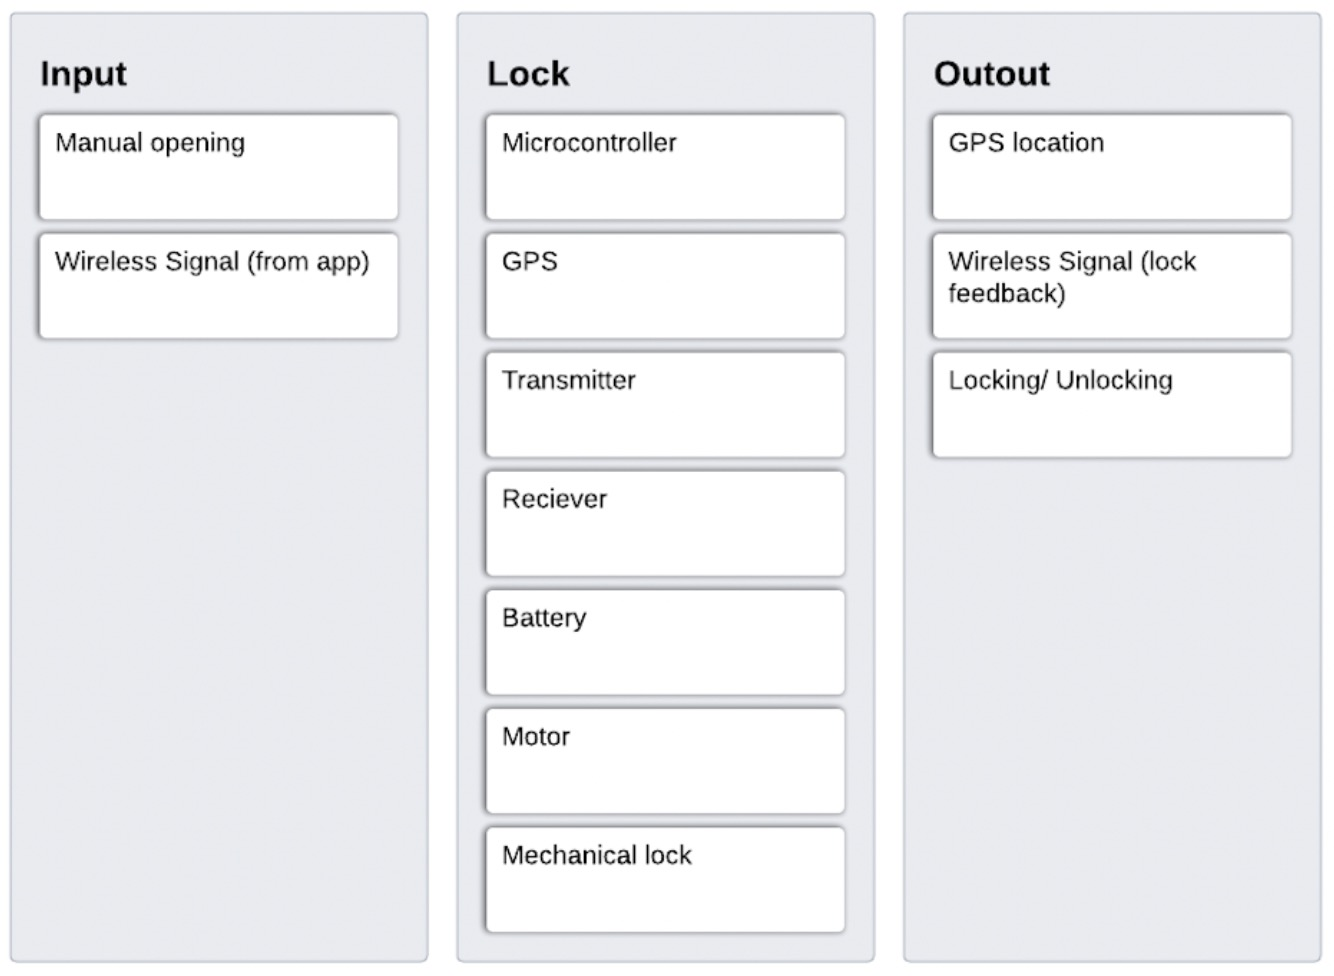
\includegraphics[width=0.6\linewidth]{../SystemContextDiagram.jpeg}
 }
 \caption{\label{The System Context}The System Context: Shows the inputs, the entities that manipulate them, and the outputs.}
 \end{center}
 \end{figure}

\begin{itemize}
\item User Responsibilities:
\begin{itemize}
\item Opening and Closing the physical mechanism
\item Keeping their smartphone with them and charged to be able to use the application
\item Disengaging the lock with their smartphone
\item Leaving their bike in a location where it is possible to connect to an external frame
\end{itemize}
\item \progname{} Responsibilities:
\begin{itemize}
\item Develop a mechanism(s) that closes around the wheels and connects to an external frame
\item Developing a functional lock so that users can feel secure in leaving their bike
\item Developing an App that is user-friendly that disengages the lock and stores the location of the locked bike
\end{itemize}
\end{itemize}

\subsection{User Characteristics} \label{SecUserCharacteristics}


The user of the SmartLock is anyone who owns a bike and a smartphone of any age, gender or biking ability.  The locking mechanism of the SmartLock functions similarly to that of any other locking device so that no special skills are required to perform the engagement/disengagement of the lock.  The physical mechanism is designed to be simple so that anyone who has the dexterity and physical strength to ride a bike will have the capability to open and close it with no strain.  The application needs to be on a smartphone that supports Bluetooth v4.0 or higher (ie. any iPhone 4S or newer or any Android with OS 4.3 or newer), the user will be expected to understand how basic applications work on these devices.  However, the application itself will be designed to be user-friendly and simple so that the functionality is clear and users do not have to spend lots of time learning the App, and the use time of the App when locking your bike is short. 

\subsection{System Constraints}

The system has the following constraints.

\begin{itemize}

\item[SC\refstepcounter{scnum}\thescnum\label{SC1}:] The project must be completed before the demo date.

\item[SC\refstepcounter{scnum}\thescnum\label{SC2}:] The materials and resources used to design and build the project must be accessible to students.
	\begin{itemize}
		\item Justification: The materials and resources are not available only to professionals or businesses and they cannot be industrial grade, i.e. they must be available at accessible local businesses.
	\end{itemize} 

\item[SC\refstepcounter{scnum}\thescnum\label{SC3}:] The budget for testing, designing, and equipment is \$750.
	\begin{itemize}
		\item Justification: The project has a finite budget to work within to encourage the efficient use of materials and ensure low costs.
	\end{itemize} 
	
\item[SC\refstepcounter{scnum}\thescnum\label{SC4}:]  The project must be mounted on existing bike designs.
	\begin{itemize}
		\item Justification: The team does not have the ability to design a custom bike to mount the project on. 
	\end{itemize} 	
	
\item[SC\refstepcounter{scnum}\thescnum\label{SC5}:] The project must be locked on existing external locking frames or racks.
	\begin{itemize}
		\item Justification: The team does not have the ability to design a custom bike rack to lock the project to. 
	\end{itemize} 

\end{itemize}

\subsection{Normal Use Cases}
In general, for a normal use case, the user will manually close the lock frame. Then, the SmartLock system must be able to disengage the SmartLock remotely through the SmartLock mobile interface after which the user must be able to open the SmartLock.  The SmartLock must also be able to send "bike parked” location coordinates as well as current SmartLock statuses back to the mobile application. 
\subsubsection{Lock is Engaged/Disengaged}
The lock is to be disengaged through the SmartLock mobile application.  Given that the user is within range of the system, the SmartLock is designed to receive the corresponding signal request from the user’s smartphone and perform the corresponding action of disengaging the lock.  The system then sends the current engaged/disengaged status to the mobile application for the user to view.
\subsubsection{Lock is Open/Closed}
Once the request to disengage the lock is sent, the system is not designed to perform the swing action of the lock. The system is designed to accept the user’s manual input of swinging the lock to the desired open/closed position.  
\subsubsection{SmartLock location is requested}
The user’s smartphone's current coordinates can be requested through the mobile application by the user.  When the user is near the lock, then they can tag their coordinates, for later use if they forget where their bike is locked.  

\section{Specific System Description}


\subsection{Problem Description} \label{Sec_pd}

There are many problems associated with bike locks today.  People often forget or lose their keys, lock or combination.  Additionally, current locking systems are often not comprehensive – they may not lock all parts of the bike that can be stolen, namely the seat, front and back wheels, and frame.  


Furthermore, bike locks can be bulky, heavy and dangerous to carry around. It can also be tedious to find and lock one’s bike to an external frame.  The combination of these nuisances can lead to individuals leaving their bikes without properly securing them.  The city of Toronto reports an average of 3625 stolen bikes annually, and the Canadian Cycling Magazine estimates that only 15-20\% of stolen bikes are reported, which indicates a rather expansive problem that can be solved [1,2].  

\subsubsection{Terminology and  Definitions}

The terms listed below will be used throughout the scope of this document and should be referenced when referring to specific components.  

\begin{itemize}
\item SmartLock: The scope of this project and document refers to both the mechanical lock and the mobile application communicating with it. 
\item Lock: The physical component of the SmartLock; includes the hardware, battery, motor, and locking mechanism.  
\item Team: The authors of this document.
\item App: The mobile application used to communicate with the lock.
\item Open/Close: The process of physically moving the lock frame into a state where it can be latched onto something else. 
\item Engage/Disengage: The automated process to actuate the lock to secure the frame. 
\item Wireless Signalling: The means of communication between the lock and the mobile application. 
\item Battery: The power source used to power the motor for engaging and disengaging. 
\item Battery Status: A measure of the quantity of charge in the battery. 
\item Git: The platform used to store the documentation and software and track changes made to the files. 
\item XCode and Flutter: The IDE used to develop the mobile application. 
\item Cross-Platform Development: The means of developing the mobile application on both iOS and Android devices. 
\item Transmitter: The device is used to send signals to and from the App to give status information and to send the engagement and disengagement signals. 
\item GPS: The satellite-based navigation system used to locate the bike. 
\item Receiver: The device used to receive the signals from the App for engagement and disengagement. 
\item Microcontroller: The programmable device used to control the motor. 
\end{itemize}
~\newpage
\subsubsection{Physical System Description} \label{sec_phySystDescrip}
~\newline
 \begin{figure}[h!]
 \begin{center}
 %\rotatebox{-90}
 {
 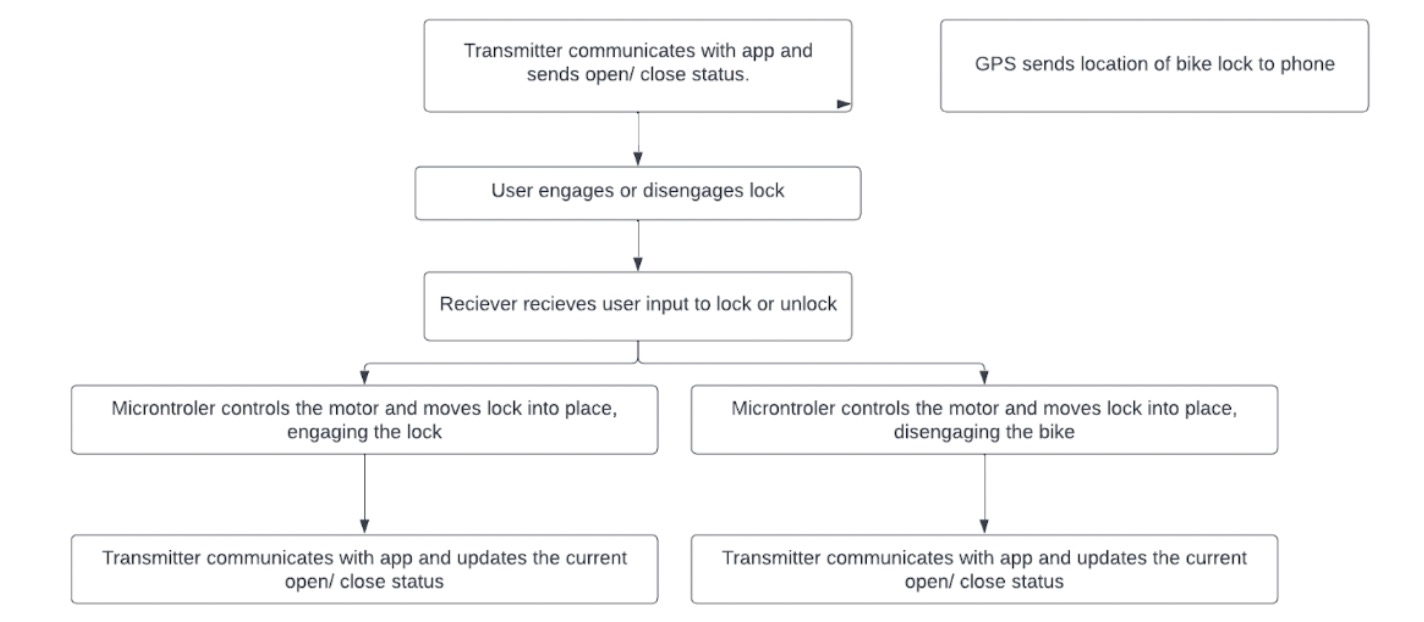
\includegraphics[width=0.6\linewidth]{../FunctionalDiagram.jpeg}
 }
 \caption{\label{The Physical System} The Physical System}
 \end{center}
 \end{figure}

\subsubsection{Assumptions} \label{sec_assumpt}

\begin{itemize}

\item A1: The user’s smartphone will always be able to connect to the project (wireless connection works as intended).
	\begin {itemize}
		\item Dependencies: All users have modern phones that can operate the App. The phones will also have functional location settings.  
	\end {itemize}
	
\item A2: Users will have no limiting physical disabilities.
	\begin {itemize}
		\item Dependencies: The average person is strong enough to manually lock and unlock the bike.
	\end {itemize}
	
\item A3: The lock will be weatherproof.
	\begin {itemize}
		\item Dependencies: Rain, snow or extreme temperatures will not damage the lock. 
	\end {itemize}
	
\item A4: Battery life is only reduced when the motor is being used.
	\begin {itemize} 
		\item Dependencies: Battery life is independent of weather and time.
	\end {itemize}

\item A5: Battery efficiency is always constant.
	\begin {itemize}
		\item Dependencies: The battery's power does not decrease over time.
	\end {itemize}
	
\item A6: The user is responsible for manually locking and unlocking the lock frame. The locking mechanism will be automatically engaged when the lock frame is locked.
	\begin {itemize}
		\item Dependencies: The user is physically capable of putting into place and removing the lock frame.
	\end {itemize}


\end{itemize}


\subsubsection{Theoretical Models}\label{sec_theoretical}

\noindent
\deftheory
% #2 refname of theory
% #3 label
{Torque of a Motor}
% #4 equation
{
  ${\bf T = F \cdot d} = {\bf I  \cdot  k_T}$
}

% #5 description
{
The above equation gives the torque $T$ (\si{\newton\metre}) required to actuate the opening and closing mechanism of the lock through the motor. Torque is equal to the force $F$ (\si{\newton}) to open or close the lock, multiplied by the distance $d$ (\si{\metre}) from the motor's axis of rotation. To extract current, torque is also equal to the load (motor) current $I$ (\si{\ampere}) multiplied by the motor's torque Constant $k_T$ (\si{\newton\metre\per\ampere}).  

The net force will be calculated once the design is finalized. The distance and torque constant will be dependent on the motor. These equations will be used to calculate the current required from the battery. They must be computed twice; once for engaging, and again for disengaging. 
}
% #6 Notes
{
None.
}
% #7 Source
{
  \url{https://www.motioncontroltips.com/faq-whats-the-relationship-between-current-and-dc-motor-output-torque/ }
}
% #8 Referenced by
{
  None
}
% #9 Preconditions
{
None
}
% #1 derivation - not applicable by default
{}

\noindent
\deftheory
% #2 refname of theory
% #3 label
{Ohm's Law}
% #4 equation
{
  $V = I \cdot R$
}

% #5 description
{
The above equation gives the voltage $V$ (\si{\volt}), which is equal to the load (motor) current $I$ (\si{\ampere}) multiplied by the resistance $R$ (\si{\ohm}) of the motor. This can be used to find the rating of the battery needed to power the motor. This calculation must also be done twice as outlined above.
}
% #6 Notes
{
None.
}
% #7 Source
{

}
% #8 Referenced by
{
None
}
% #9 Preconditions
{
None
}
% #1 derivation - not applicable by default
{}

~\newline

\noindent
\deftheory
% #2 refname of theory
% #3 label
{Battery Life}
% #4 equation
{
  ${\bf BL = \frac{BC}{I}}$
}

% #5 description
{
The above equation gives the battery life $BL$ (\si{\hour}), which will be calculated by dividing the battery capacity $BC$ (\si{\ampere\hour}) selected and the load current $I$ (\si{\ampere)}.
}
% #6 Notes
{
None.
}
% #7 Source
{
 
}
% #8 Referenced by
{
None
}
% #9 Preconditions
{
None
}
% #1 derivation - not applicable by default
{}

~\newpage
\section{Requirements}

This section provides the functional requirements, the business tasks that the software is expected to complete, and the nonfunctional requirements, the qualities that the software is expected to exhibit.

\subsection{Functional Requirements}

\subsubsection{User Input Related}
\begin{itemize}
\setlength{\itemindent}{.5in}
\item[FR\refstepcounter{reqnum}\thereqnum\label{FRDisengage}:] LockDisengage input must disengage the lock on the bike.
\\ \-\ \-\ \-\ \-\ \-\ \-\ \-\ \-\ Rationale: When the unlock button of the App is pressed to disengage the lock, the bike lock must be disengaged.
\item[FR\refstepcounter{reqnum}\thereqnum\label{FRLockStatusEngaged}:] When the lock is engaged, the lock status must read engaged.
\\ \-\ \-\ \-\ \-\ \-\ \-\ \-\ \-\ Rationale: The App must output the correct status as engaged when engaged.
\item[FR\refstepcounter{reqnum}\thereqnum\label{FRLockStatusDisengaged}:] When the lock is disengaged, the lock status must read disengaged.
\\ \-\ \-\ \-\ \-\ \-\ \-\ \-\ \-\ Rationale: The App must output the correct status as disengaged when disengaged.
\item[FR\refstepcounter{reqnum}\thereqnum\label{FRUserPos}:] The location of the user’s phone must be saved in the smartphone application as UserPosition.
\\ \-\ \-\ \-\ \-\ \-\ \-\ \-\ \-\ Rationale: The smartphone app must save the location of the phone so it can be displayed.
\item[FR\refstepcounter{reqnum}\thereqnum\label{FRSturdy}:] Effective Bike Lock: The lock is sturdy and cannot be manually opened by the average human once it is engaged.
\\ \-\ \-\ \-\ \-\ \-\ \-\ \-\ \-\ Rationale: If the lock is not resistant to external forces it will not be an effective lock. If the lock could be opened by the average human when engaged, then the lock would not prevent theft and be rendered useless.
\\ \-\ \-\ \-\ \-\ \-\ \-\ \-\ \-\ Verification: Apply a force between 200-400N, which is the \href{https://www.tandfonline.com/doi/pdf/10.1080/10803548.2004.11076594?cookieSet=1}{average human's arm strength}, to pry open the lock over fifty trials. 
\item[FR\refstepcounter{reqnum}\thereqnum\label{FRCorrectUser}:] The lock must only be engaged/disengaged by the intended user(s).
\\ \-\ \-\ \-\ \-\ \-\ \-\ \-\ \-\ Rationale: Not everyone with the App can engage/disengage the lock on your bike to provide added security.
\end{itemize}

\subsubsection{Bike Input Related}
\begin{itemize}
\setlength{\itemindent}{.5in}
\item[FR\refstepcounter{reqnum}\thereqnum\label{FRBikeFrame}:] The lock can be mounted to the bike's frame.
\\ \-\ \-\ \-\ \-\ \-\ \-\ \-\ \-\ Rationale: If the lock can not be mounted to the user's bike it will not be effective as a lock.
\end{itemize}

\subsubsection{Output Related}
\begin{itemize}
\setlength{\itemindent}{.5in}
\item[FR\refstepcounter{reqnum}\thereqnum\label{FRBatteryLevelDisplay}:] Battery level must be displayed on the App.
\\ \-\ \-\ \-\ \-\ \-\ \-\ \-\ \-\ Rationale: The user must be able to view the battery level in order to know when the battery requires replacement.
\item[FR\refstepcounter{reqnum}\thereqnum\label{FRLocDisplay}:] The location of the bike must be shown on the App as BikePosition.
\\ \-\ \-\ \-\ \-\ \-\ \-\ \-\ \-\ Rationale: The user must be able to view the location of their bike so that they can find their bike upon returning to it.
\item[FR\refstepcounter{reqnum}\thereqnum\label{FRPower}:] The battery must output enough power to disengage the lock.
\\ \-\ \-\ \-\ \-\ \-\ \-\ \-\ \-\ Rationale: The locking system will not be functional if the battery is not able to disengage the lock.
\end{itemize}

\subsection{Nonfunctional Requirements}

\subsubsection{Smart Phone}
\begin{itemize}
\setlength{\itemindent}{.5in}
\item[NFR\refstepcounter{nfrnum}\thenfrnum\label{NFRInst}:] Can reasonably be used without requiring an instruction manual.
\\ \-\ \-\ \-\ \-\ \-\ \-\ \-\ \-\ Rationale: The system must be easy to use with a minimal learning curve for it to be useful.
\\ \-\ \-\ \-\ \-\ \-\ \-\ \-\ \-\ Verification: The App will be verified by test users, and the learning period will be tracked
\item[NFR\refstepcounter{nfrnum}\thenfrnum\label{NFRStor}:] App storage must be under fifty megabytes. A small mobile app should not take up significant space on the user's phone.
\\ \-\ \-\ \-\ \-\ \-\ \-\ \-\ \-\ Rationale: The App should fit on anyone's phone, and use up minimal storage.
\end{itemize}

\subsubsection{Physical Design}
\begin{itemize}
\setlength{\itemindent}{.5in}
\item[NFR\refstepcounter{nfrnum}\thenfrnum\label{NFRVisual}:] The design must be visually appealing.
\\ \-\ \-\ \-\ \-\ \-\ \-\ \-\ \-\ Rationale: The lock must be visually appealing in order for it to be a desirable product.
\\ \-\ \-\ \-\ \-\ \-\ \-\ \-\ \-\ Verification: The design will be verified by test users who will rank how visually  appealing the lock is.
\item[NFR\refstepcounter{nfrnum}\thenfrnum\label{NFRFunc}:] The design must not impede normal bike functions.
\\ \-\ \-\ \-\ \-\ \-\ \-\ \-\ \-\ Rationale: The lock will not be used if it negatively impacts the normal function of the bike.
\\ \-\ \-\ \-\ \-\ \-\ \-\ \-\ \-\ Verification: Lock will be verified by mounting it on test users' bikes, then having them use the bike.
\item[NFR\refstepcounter{nfrnum}\thenfrnum\label{NFRHarm}:] The design must not inflict harm to the user in any way, such as clamping down on a finger, or moving at a force or speed that could cause injury. 
\\ \-\ \-\ \-\ \-\ \-\ \-\ \-\ \-\ Rationale: It is undesireable for the lock to inflict harm to the user.
\\ \-\ \-\ \-\ \-\ \-\ \-\ \-\ \-\ Verification: Lock will be verified by ensuring there are no automatically moving parts that can come into contact with the user, (i.e. they are hidden). 

\end{itemize}

\subsubsection{Accuracy}
\begin{itemize}
\setlength{\itemindent}{.5in}
\item[NFR\refstepcounter{nfrnum}\thenfrnum\label{NFRAccuracyStatus}:] The accuracy of the bike lock status must be above 95\%.
\\ \-\ \-\ \-\ \-\ \-\ \-\ \-\ \-\ Rationale: The status must report the correct status in order to function optimally. The figure of 95\% was taken as it is the most common confidence interval used. 
\\ \-\ \-\ \-\ \-\ \-\ \-\ \-\ \-\ Verification: The status will be manually verified over 100 trials. 
\item[NFR\refstepcounter{nfrnum}\thenfrnum\label{NFRAccuracyPos}:] Where location services are available, the accuracy of location coordinates must be within 10m.
\\ \-\ \-\ \-\ \-\ \-\ \-\ \-\ \-\ Rationale: For the locating feature to be useful, it must be accurate. The figure of 10m was obtained since a bike within a distance of 10m will be visible. 
\\ \-\ \-\ \-\ \-\ \-\ \-\ \-\ \-\ Verification: The accuracy of location coordinates will be manually verified over fifty trials. 
\item[NFR\refstepcounter{nfrnum}\thenfrnum\label{NFRBatteryLevel}:] Battery level must be calculated accurately within 10\%.
\\ \-\ \-\ \-\ \-\ \-\ \-\ \-\ \-\ Rationale: To avoid a situation where the battery dies unbeknownst to the user, the battery level must be accurate. The average user would replace their battery when it only has 10\% charge left.
\\ \-\ \-\ \-\ \-\ \-\ \-\ \-\ \-\ Verification: Observe the battery charge shown right before the battery dies. 
\end{itemize}

\subsubsection{Usability}
\begin{itemize}
\setlength{\itemindent}{.5in}
\item[NFR\refstepcounter{nfrnum}\thenfrnum\label{NFRCompQuick}:]  The SmartLock must be quicker to use than a typical keyed or combination bike lock.
\\ \-\ \-\ \-\ \-\ \-\ \-\ \-\ \-\ Rationale: If using the SmartLock takes longer than a typical lock, it is no more convenient than a typical lock, which is a key selling feature. 
\\ \-\ \-\ \-\ \-\ \-\ \-\ \-\ \-\ Verification: The use of both the SmartLock and a key and combination lock by the average user will be timed and compared. 
\item[NFR\refstepcounter{nfrnum}\thenfrnum\label{NFRCompForce}:] Opening and closing the lock frame must require similar force to a typical keyed or combination lock.
\\ \-\ \-\ \-\ \-\ \-\ \-\ \-\ \-\ Rationale: If opening and closing the lock takes more strength than a typical lock, it is no longer convenient for the user. 
\\ \-\ \-\ \-\ \-\ \-\ \-\ \-\ \-\ Verification: Measure the force required to use a typical keyed and combination lock, then measure force required for the SmartLock and compare.
\item[NFR\refstepcounter{nfrnum}\thenfrnum\label{NFRBatteryLife}:] The battery must last for greater than one month and/or sixty rides before needing to be replaced or charged.
\\ \-\ \-\ \-\ \-\ \-\ \-\ \-\ \-\ Rationale: It would be inconvenient to ask for the user to replace the batteries more frequently than this.
\item[NFR\refstepcounter{nfrnum}\thenfrnum\label{NFRBatteryAccess}:] Batteries must be accessible to replace or chargeable.
\\ \-\ \-\ \-\ \-\ \-\ \-\ \-\ \-\ Rationale: If the batteries are not accessible to replace or charge, then when the battery dies initially, the user can no longer use the SmartLock.
\item[NFR\refstepcounter{nfrnum}\thenfrnum\label{NFRTools}:] The lock must be easily mounted on the bike frame. It does not require special tools (those not found in a typical toolbox, such as power tools) to be installed and doing so does not take more than twenty minutes. 
\\ \-\ \-\ \-\ \-\ \-\ \-\ \-\ \-\ Rationale: Required for convenience for user. 
\item[NFR\refstepcounter{nfrnum}\thenfrnum\label{NFRModels}:] The lock can be used for many different models of mountain, city, and road bikes. 
\\ \-\ \-\ \-\ \-\ \-\ \-\ \-\ \-\ Rationale: The SmartLock must fit a wide variety of bikes so that is is accessible to be used with most users' bikes.
\\ \-\ \-\ \-\ \-\ \-\ \-\ \-\ \-\ Verification: Test the SmartLock on as many different bikes as accessible. Ensure that this range includes all typical bike frame dimensions and shapes. For those not accessible, compare the dimensions of a typical bike frame, (frame length of 17 inches), with the dimensions/shape of the SmartLock to ensure the lock can be used. 
\end{itemize}

\subsubsection{Maintainability}
Changes to the items below should take less than X\_FRACTION of total development time.
\\ Rationale: This rationale applies to all of the requirements in this subsection. In order for the lock to be used for a long period of time, when it breaks or needs improvements, maintenance must be able to be made. 
\begin{itemize}
\setlength{\itemindent}{.5in}
\item[NFR\refstepcounter{nfrnum}\thenfrnum\label{NFRGUI}:] GUI\_FRACTION, Making changes to the GUI.
\item[NFR\refstepcounter{nfrnum}\thenfrnum\label{NFRController}:] CONTROLLER\_FRACTION, Arduino/Electromagnet Controller Software.
\item[NFR\refstepcounter{nfrnum}\thenfrnum\label{NFRCircuit}:] ELCTRICAL\_FRACTION, Electrical Circuit.
\item[NFR\refstepcounter{nfrnum}\thenfrnum\label{NFRMech}:] MECHANICAL\_FRACTION, Mechanical physical design.
\end{itemize}

\subsubsection{Portability}
\begin{itemize}
\setlength{\itemindent}{.5in}
\item[NFR\refstepcounter{nfrnum}\thenfrnum\label{NFRPortability}:] The App should run on iOS and Android.
\\ \-\ \-\ \-\ \-\ \-\ \-\ \-\ \-\ Rationale: Most smartphones use these platforms, allowing the system to be accessible to the majority of people.
\item[NFR\refstepcounter{nfrnum}\thenfrnum\label{NFRUpdates}:] The App should be easily maintained through smartphone software updates.
\\ \-\ \-\ \-\ \-\ \-\ \-\ \-\ \-\ Rationale: The App should be able to be used even when a user updates their phone.
\\ \-\ \-\ \-\ \-\ \-\ \-\ \-\ \-\ Verification: Maintenance to the App in preparation for OS updates must be less than the initial development time. Maintenance will be done for every OS update to ensure the App runs on the updated OS for both iPhone and Android smartphones.


\end{itemize}

%\subsubsection{Security}
%\begin{itemize}
%\setlength{\itemindent}{.5in}

%I moved the requirement that was in this section to be a functional requirement --Abi

%\end{itemize}

\section{Likely Changes}    

\begin{itemize}

\item[LC\refstepcounter{lcnum}\thelcnum\label{LC_meaningfulLabel}:]  Depending on the battery life, showing battery level on the App, as required in \hyperref[FRBatteryLevelDisplay]{FR8}, might not be necessary. If the battery life is very long, then perhaps a warning that the battery is low is sufficient. 
\item[LC\refstepcounter{lcnum}\thelcnum\label{LC_meaningfulLabel}:] Having never created an app like this before, the amount of storage needed for the App is unknown. Requirement \hyperref[NFRStor]{NFR2} provides ample space, if any change, this requirement might be revised so that it be required that the App takes up even less storage. 
\item[LC\refstepcounter{lcnum}\thelcnum\label{LC_meaningfulLabel}:] Even though aesthetics is a selling point of any product, it is not a priority for this product. As such, the requirement \hyperref[NFRVisual]{NFR3} is subject to change. 
\item[LC\refstepcounter{lcnum}\thelcnum\label{LC_meaningfulLabel}:] The degree of accuracy mentioned in \hyperref[NFRAccuracyStatus]{NFR6}, \hyperref[NFRAccuracyPos]{NFR7}, and \hyperref[NFRBatteryLevel]{NFR8}
\item[LC\refstepcounter{lcnum}\thelcnum\label{LC_meaningfulLabel}:] Given that we will likely not be maintaining the system, requirements regarding maintainability will be difficult to test and verify. While products should be designed with maintainability in mind, it is not a priority for this project. Thus, requirements \hyperref[NFRGUI]{NFR15}, \hyperref[NFRController]{NFR16}, \hyperref[NFRCircuit]{NFR17}, \hyperref[NFRMech]{NFR18} are subject to change. 

\end{itemize}

\section{Unlikely Changes}    

\noindent \begin{itemize}

\item[ULC\refstepcounter{ulcnum}\theulcnum\label{LC_meaningfulLabel}:] These requirements are core to the functionality of the product. The product would not accomplish its purpose without meeting these requirements. Thus, these requirements are  unlikely to change: \hyperref[FRDisengage]{FR1}, \hyperref[FRLockStatusEngaged]{FR2}, \hyperref[FRLockStatusDisengaged]{FR3}, \hyperref[FRUserPos]{FR4}, \hyperref[FRSturdy]{FR5}, \hyperref[FRCorrectUser]{FR6}, \hyperref[FRPower]{FR10}.
\item[ULC\refstepcounter{ulcnum}\theulcnum\label{LC_meaningfulLabel}:] These requirements are key selling features of the system, and are therefore unlikely to change: \hyperref[FRBikeFrame]{FR7}, \hyperref[FRBatteryLevelDisplay]{FR8}.
\item[ULC\refstepcounter{ulcnum}\theulcnum\label{LC_meaningfulLabel}:] These requirements are necessary to ensure accessibility for all users: \hyperref[NFRInst]{NFR1}.
\item[ULC\refstepcounter{ulcnum}\theulcnum\label{LC_meaningfulLabel}:] Dependent on requirement \hyperref[FRBikeFrame]{FR7}, that the lock can be mounted on the bike's frame, \hyperref[NFRFunc]{NFR4} that the design must not impede normal bike function is necessary for the bike to function at all, and, if the bike does not function, the SmartLock product is useless. As such, this requirement is unlikely to change.
\item[ULC\refstepcounter{ulcnum}\theulcnum\label{LC_meaningfulLabel}:] The following requirements must be satisfied to maintain an edge over typical, manually engaged/disengaged bike locks, and are therefore unlikely to change: \hyperref[NFRCompQuick]{NFR9}, \hyperref[NFRCompForce]{NFR10}, \hyperref[NFRBatteryLife]{NFR11},  \hyperref[NFRBatteryAccess]{NFR12}, \hyperref[NFRTools]{NFR13}, \hyperref[NFRModels]{NFR14}.

\end{itemize}

\section{Traceability Index}

The following list will take the following form:
\\The first requirement: is dependent on the following list of requirements/constraints/assumptions
\\
/monitored variables and vice versa
\\
 \\  \hyperref[FRDisengage]{FR1}: \hyperref[FRLockStatusDisengaged]{FR3}, MV2
\\  \hyperref[FRSturdy]{FR5}: \hyperref[FRLocDisplay]{FR9}, \hyperref[NFRAccuracyPos]{NFR7}, MV4
\\  \hyperref[FRBikeFrame]{FR7}: \hyperref[NFRTools]{FR13}, \hyperref[NFRModels]{FR14}, SC4
\\  \hyperref[FRBatteryLevelDisplay]{FR8}: \hyperref[FRPower]{FR10},\hyperref[NFRBatteryLevel]{NFR8}, MR6
\\  \hyperref[NFRStor]{NFR2}: \hyperref[NFRGUI]{NFR15}
\\  \hyperref[NFRVisual]{NFR3}: \hyperref[NFRFunc]{NFR4}
 \\  \hyperref[NFRCompQuick]{NFR9}: \hyperref[NFRBatteryLife]{NFR11}, A1
 \\  \hyperref[NFRTools]{NFR13}: A4, A5
\section{Development Plan: Prioritizing and Phasing of Requirements}

%\plt{This section is optional.  It is used to explain the plan for developing
 % the software.  In particular, this section gives a list of the order in which
 % the requirements will be implemented.  In the context of a course, this is
 % where you can indicate which requirements will be implemented as part of the
 % course, and which will be ``faked'' as future work.  This section can be
 % organized as a prioritized list of requirements, or it could the
 % requirements that will be implemented for ``phase 1'', ``phase 2'', etc.}

\subsection{Phase 1}
Phase 1 consists of implementing requirements that, together, make up the minimum viable product: a lock that can be engaged remotely. These requirements are the highest priority and should be completed first, throughout November and December. These requirements include:
\hyperref[FRDisengage]{FR1}, \hyperref[FRLockStatusEngaged]{FR2}, \hyperref[FRLockStatusDisengaged]{FR3}, \hyperref[FRCorrectUser]{FR6}.

\subsection{Phase 2}
Phase 2 consists of requirements informing the design of the minimum viable product of the physical bike lock. These are the second highest priority but will be completed in parallel with Phase 1 requirements. These requirements include:
\hyperref[FRSturdy]{FR5}, \hyperref[FRBikeFrame]{FR7}, \hyperref[FRPower]{FR10}, \hyperref[NFRFunc]{NFR4}, \hyperref[NFRBatteryLife]{NFR11}, \hyperref[NFRTools]{NFR13},\hyperref[NFRModels]{NFR14}.

\subsection{Phase 3}
Phase 3 consists of requirements regarding the locating feature. These are lower priorities, but key selling features. These requirements will be completed after Phase 1 and Phase 2, in January. These requirements include:
\hyperref[FRUserPos]{FR4}, \hyperref[FRLocDisplay]{FR9}.

\subsection{Phase 4}
Phase 4 consists of requirements that ensure the accuracy, usability, and accessibility of features. This phase will be completed after Phase 3, likely in February. These requirements include:
\hyperref[FRBatteryLevelDisplay]{FR8}, \hyperref[NFRInst]{NFR1}, \hyperref[NFRStor]{NFR2},  \hyperref[NFRHarm]{NFR5}, \hyperref[NFRAccuracyStatus]{NFR6}, \hyperref[NFRAccuracyPos]{NFR7}, \hyperref[NFRBatteryLevel]{NFR8}, \hyperref[NFRCompQuick]{NFR9}, \hyperref[NFRBatteryLife]{NFR11}, \hyperref[NFRBatteryLife]{NFR11}, \hyperref[NFRBatteryAccess]{NFR12}.

\subsection{Phase 5}
Phase 5 consists of requirements regarding the aesthetics of the product, and is the lowest priority. These requirements include: \hyperref[NFRVisual]{NFR3}.

\subsection{Phase 6}
Phase 6 consists of requirements that ensure maintainability, which is likely outside of the scope of this project. These requirements include: \hyperref[NFRGUI]{NFR15}, \hyperref[NFRController]{NFR16}, \hyperref[NFRCircuit]{NFR17}, \hyperref[NFRMech]{NFR18}.

\section{Values of Auxiliary Constants}

\begin{itemize}
\setlength{\itemindent}{0.5in} \item[CONST\refstepcounter{constnum}\theconstnum\label{LC_meaningfulLabel}:] GUI\_CONSTANT = 0.3, \hyperref[NFRGUI]{NFR15}
\item[CONST\refstepcounter{constnum}\theconstnum\label{LC_meaningfulLabel}:] CONTROLLER\_CONSTANT = 0.3, \hyperref[NFRController]{NFR16}
\item[CONST\refstepcounter{constnum}\theconstnum\label{LC_meaningfulLabel}:] ELECTRICAL\_CONSTANT = 0.3, \hyperref[NFRCircuit]{NFR17}
\item[CONST\refstepcounter{constnum}\theconstnum\label{LC_meaningfulLabel}:] MECHANICAL\_CONSTANT = 0.3, \hyperref[NFRMech]{NFR18}
\end{itemize}

\newpage

\bibliographystyle {plainnat}
\bibliography {../../refs/References}

\newpage

\newpage{}
\section{Appendix A}

\subsection{Table of Monitored Variables}

\begin{minipage}{\textwidth}
\renewcommand*{\arraystretch}{1.5}
\begin{tabular}{| p{0.23\textwidth} | p{0.54\textwidth} | p{0.08\textwidth} | p{0.15\textwidth} |}
 \hline
 Variable Name & Description & Type & Units \\ 
 \hline
 m\_SignalEngaged & Monitors whether or not the locking mechanism is engaged & Digital & Boolean \\ 
  \hline
 m\_SignalDisengaged & Monitors whether or not the locking mechanism is disengaged & Digital & Boolean \\ 
  \hline
 m\_Location & Monitors the location of the bike & Analog & Coordinates \\ 
  \hline
 m\_BatteryPower & Monitors the current battery level & Analog & Level \\ 
 \hline
\end{tabular}
\end{minipage}\\

\subsection{Table of Controlled Variables}

\begin{minipage}{\textwidth}
\renewcommand*{\arraystretch}{1.5}
\begin{tabular}{| p{0.25\textwidth} | p{0.52\textwidth} | p{0.08\textwidth} | p{0.15\textwidth} |}
 \hline
 Variable Name & Description & Type & Units \\ 
  \hline
 c\_LocklDisengaged & Disengages the lock & Digital & Boolean \\ 
  \hline
 c\_LockOpen & Indicates to the user that the latch is open & Digital & Boolean \\ 
  \hline
 c\_LockClosed& Indicates to the user that the latch is closed & Digital & Boolean \\ 
  \hline
 c\_BikePosition & Marks the location of the bike when it is locked & Analog & Coordinates \\ 
  \hline
 c\_BatteryLevelStatus & Indicates the level of the battery & Analog & Level \\ 
 \hline
\end{tabular}
\end{minipage}\\
~\newline
\subsection{Constants -- NA}
~\newline
%%
\subsection{Stimulus and Responses}
~\newline
\begin{figure}[h!]
 \begin{center}
 {
 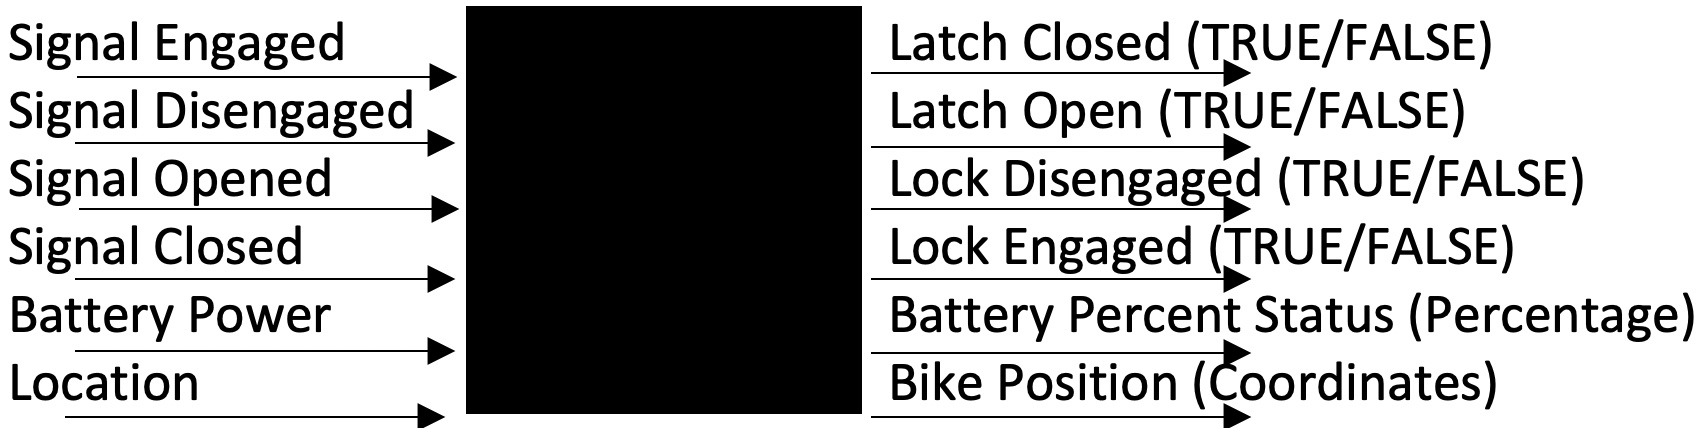
\includegraphics[width=0.6\linewidth]{./StimulusandResponses.jpeg}
 }
 \caption{\label{Stimulus and Responses} Stimulus and Responses}
 \end{center}
 \end{figure}
%%
\subsection{Notation}
~\newline
\begin{figure}[h!]
 \begin{center}
 {
 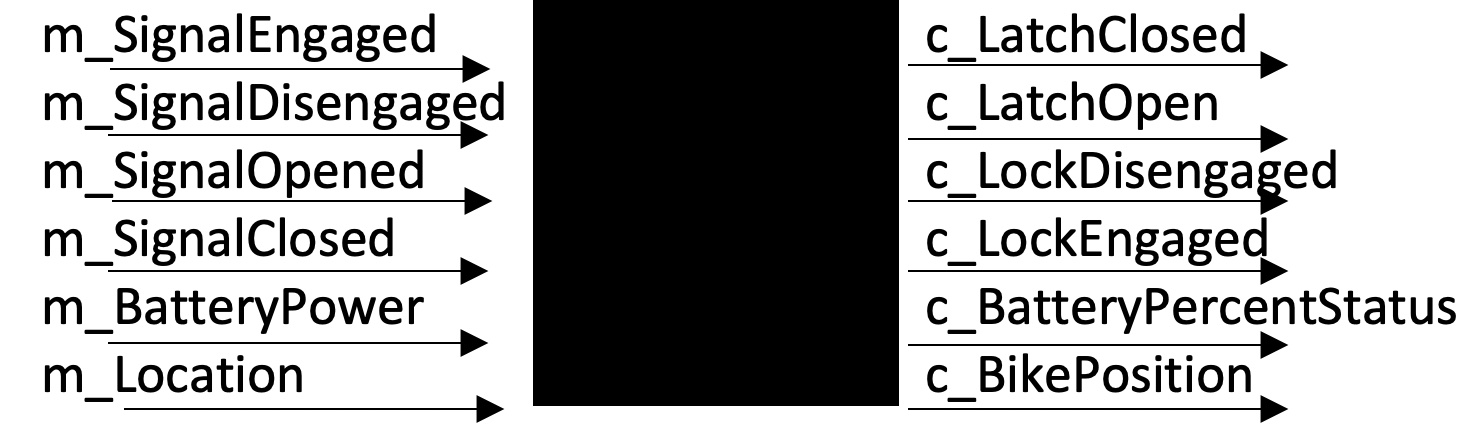
\includegraphics[width=0.6\linewidth]{./Notation.jpeg}
 }
 \caption{\label{Notation} Notation}
 \end{center}
 \end{figure}
%%
~\newpage
\subsection{Responses}
~\newline
\begin{figure}[h!]
 \begin{center}
 {
 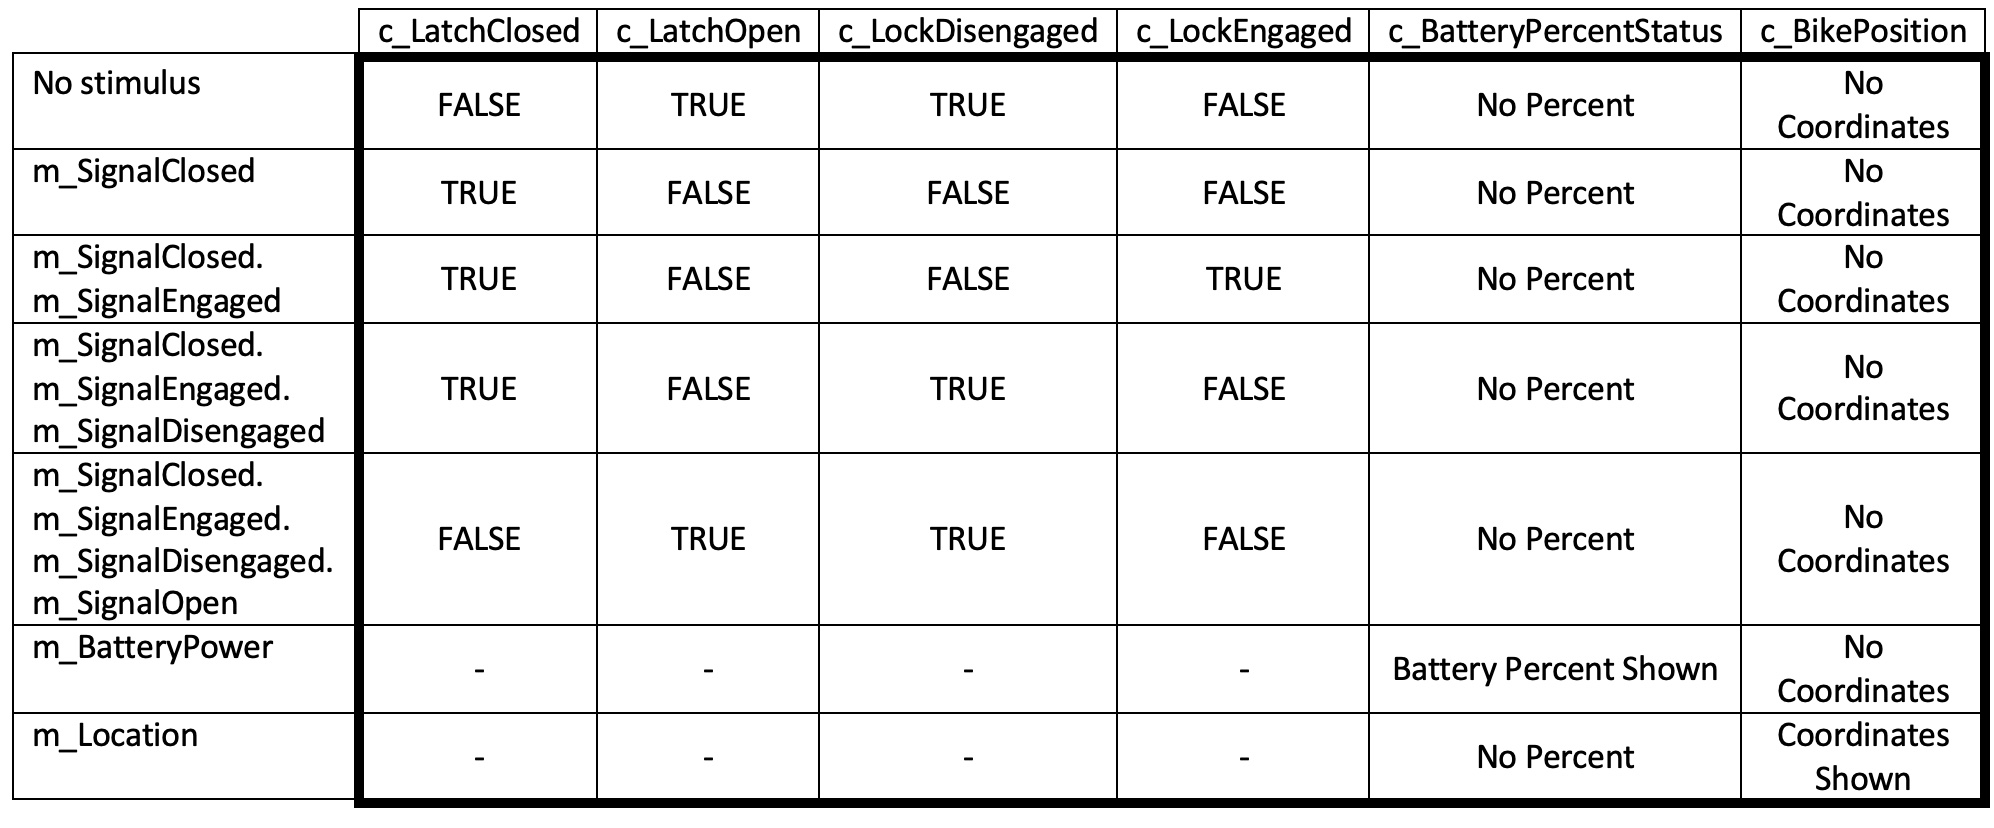
\includegraphics[width=0.9\linewidth]{./Responses.jpeg}
 }
 \caption{\label{Responses} Responses}
 \end{center}
 \end{figure}
%%
\subsection{Effect of Each Stimulus}
~\newline
\begin{figure}[h!]
 \begin{center}
 {
 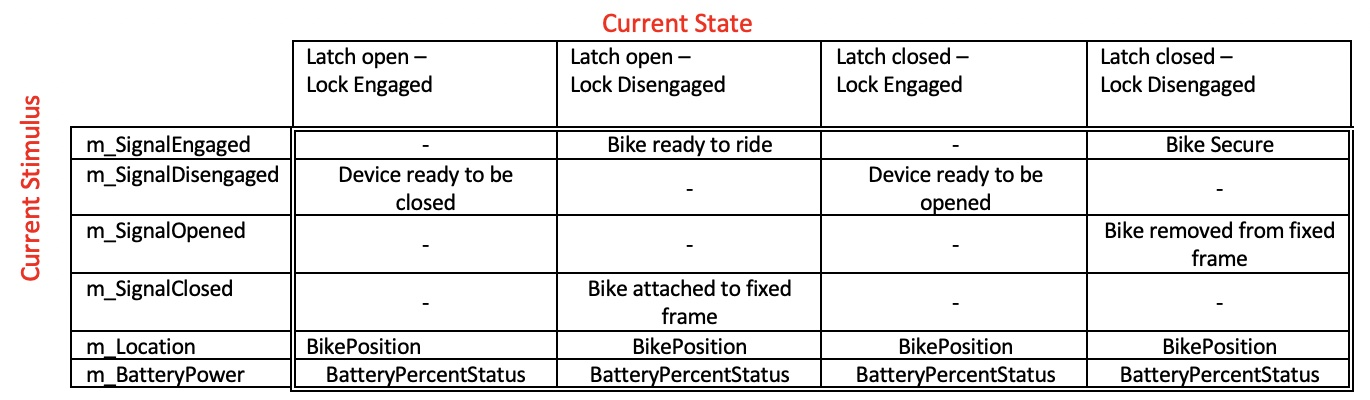
\includegraphics[width=0.9\linewidth]{./EffectofEachStimulus.jpeg}
 }
 \caption{\label{Effect of Each Stimulus} Effect of Each Stimulus}
 \end{center}
 \end{figure}
~\newpage
\section{Appendix B}
\subsection{Reflection}

The information in this section will be used to evaluate the team members on the graduate attribute of Lifelong Learning.  Please answer the following questions:

\begin{enumerate}
  \item What knowledge and skills will the team collectively need to acquire to successfully complete this capstone project?  Examples of possible knowledge to acquire include domain specific knowledge from the domain of your application, or software engineering knowledge, mechatronics knowledge or
  computer science knowledge.  Skills may be related to technology, or writing, or presentation, or team management, etc.  You should look to identify at least one item for each team member.
  ~\newline
  ~\newline
 Steffi: 
  ~\newline
My lead role on this project is regarding Documentation and Latex.  While I have experience with some project documentation, the extent to which it is necessary for this project is not something I have done before.  Looking at this project in such detail will help to more deeply understand every component of the project and help to better see the connection between every aspect.  Additionally, technical communication is a skill I have never used before so learning to use Github and Latex will be critical to the delivery of the project and developing skills that will be useful in future technical projects.
\\
\\
Abi:
\\
My lead role for this project is surrounding wireless communication, specifically Bluetooth.  I will need to learn how to implement Bluetooth communication between the SmartLock and the user's phone so that the lock can be disengaged remotely.  I have never worked with this type of technology before, so I will need to have a very steep learning curve. 
 \\
\\
Elsa:
\\ 
 I am the Embedded Systems Lead of the project, and as such I will be adding to my existing skills in order to design, build and provide support to other members of my team related to this topic. This project will require significant knowledge in the realm of electronics, wiring, microprocessor programming and general hardware systems. I am also a Support Lead of Documentation, which includes technical writing and typesetting in Latex. 
 \\
 \\
 Anthony: 
 \\
 The App will be developed using XCode Ver.14.0, utilizing the Swift programming language for iOS Development. For linting, SwiftLint will be implemented as it is commonly used in the industry for iOS development utilizing XCode. Basic background in programming is a required skill needed to be able to effectively learn the IDE and programming language.
  \\
\\
Abdul:
\\ 
 Being on the App development sub-team, I will be required to acquire a working knowledge of the Swift programming language to develop the App for the SmartLock System.  In addition to that, I would need to research Bluetooth technology and its integration within our system.
 \\
\\
Stephen:
\\
 I will need to strengthen my knowledge in many topics including mechanical prototyping/design, software development, and electrical circuit design.  I will really try to advance my knowledge in the mechanical design aspect of this project.  I will need skills to design a system that can complete its function and package all of the electrical features.  For this, I will really push my knowledge in circular prototyping and prototyping methods.
 
  \item For each of the knowledge areas and skills identified in the previous
  question, what are at least two approaches to acquiring the knowledge or
  mastering the skill?  Of the identified approaches, which will each team
  member pursue, and why did they make this choice?
    ~\newline
    ~\newline
Steffi: 
  ~\newline
 Documentation - Two approaches that I can use to improve my skillset for documentation are reading old documentation that other groups have produced, or examples of documentation online, and writing documentation and paying careful attention to the focus of the section.  The emphasis will be placed on writing documentation because with this skillset I believe the best approach is to try and then learn from what was difficult and feedback on what was produced.  However, old documentation will still be referenced as well. 
  ~\newline
  Latex - Two approaches that can be used to improve my latex skill set are referencing external explanations (videos \& Tutorials), and trial and error with external reference materials.  I will be focusing on trial and error using some external materials.  I believe that seeing what happens for yourself when you make a change is the best way to understand what is going on.  The external resources will be used to give an idea of what it is possible to try to accomplish in latex, for example, certain formatting that I may not have considered existed. 
\\
\\
Abi:
\\ There are many different approaches to learning technical skills, such as Bluetooth.  I plan to approach learning this skill by researching on the Internet, asking our supervisor for potential resources or personal knowledge, and seeking help from peers who have more knowledge on the subject.  After researching which hardware is needed to implement wireless communication, I will learn by doing, slowly building up my skills. Rather than choosing just one approach, I plan on using all of these approaches in parallel. 
\\
\\
Elsa:
\\ 
  I will acquire this expertise by learning through resources such as previous Embedded Systems and Electronics courses I have taken, online research and journals that I have access to through McMaster. Additionally, I find YouTube to be a useful experiential resource for learning how to apply acquired knowledge in personal projects. I will improve my technical writing and typesetting skills by practicing using Latex and challenging myself to continue researching and learning new modes of practice and editing.
\\
\\
Anthony:
\\
Apple has created their own modules to teach individuals how to use their IDE and programming language. Other resources include free YouTube tutorials and private companies offering courses. For the scope of this project and considering the complexity of the application, Apple’s free course and YouTube tutorials would be sufficient. Additionally, there are several public forums where individuals could search for similar problems others have experienced before and find various solutions contributed by the community. Team member Anthony Shenouda has experience with the IDE as they have developed multiple mobile applications before. They will be responsible for the overall development and ensuring the application is completed successfully and timely. 
\\
\\
Abdul:
\\ 
 Swift -  To learn Swift effectively, I plan to take a few starter courses as well as practise some basic programs using Swift. Doing so would familiarize myself with the Syntax and libraries. Most of the general programming basics I have already developed through my use of other languages. 
  
 Bluetooth - My approach to this would be to look at a few existing projects and adopt a similar approach within our system. Bluetooth is widely used, and there are a variety of open-source libraries of which we can take advantage.
\\
\\
Stephen:
\\
 To acquire the skills I need in mechanical design/prototyping I will use past course content and lecture slides from my mechanical product design, to recite the best practices for 3D printing and prototyping methods. I will also utilize the resources on campus like the Thode maker space or student workshop for direction in terms of prototyping processes as well as material selection, design, and analysis.  Finally, I will also utilize a mentor who is in the design industry to mentor me on these skills.
\end{enumerate}

\end{document}